\documentclass[compress]{beamer}

\usepackage[nofonts]{ctex}
\setCJKmainfont[ItalicFont={Kaiti SC}]{Kaiti SC}%
%\setCJKmainfont[ItalicFont={AR PL KaitiM GB}]{AR PL KaitiM GB}%
%\setCJKsansfont{WenQuanYi Zen Hei}% 文泉驿的黑体

\mode<beamer>
{
     \useinnertheme{rounded}
     \useoutertheme{split}
     \usecolortheme{rose}
     \usecolortheme{seahorse}

     \expandafter\def\expandafter\insertshorttitle\expandafter{%
       \insertshorttitle\hfill%
       \insertframenumber\,/\,\inserttotalframenumber}

}

\mode<handout>
{
	\usetheme{default}
	\usepackage{pgfpages}
	\pgfpagesuselayout{4 on 1}[a4paper,landscape,border shrink=5mm]
}


\usepackage{amsmath,latexsym,amssymb,amsfonts,amsbsy}
\usepackage{graphicx}
\usepackage{hyperref}
%\usepackage{listings}
\usepackage{fancyvrb}
\fvset{frame=single, fontsize=\small}

\newcommand{\romannumber}[1]{{\textrm{\uppercase\expandafter{\romannumeral
#1}}}}
\setbeamercolor{dblue}{fg=white,bg=blue!40!black} % for beamercolorbox
\newenvironment{pblock}{\begin{beamercolorbox}[rounded=true,
      shadow=true]{dblue}}{\end{beamercolorbox}}


\graphicspath{{figure/}}

%%%%%%%%%%%%%%%%%%%%%%%%%%%%%%%%%%%%%%%%%%%%%%%%%%%%%%%%%%%%%%%%%
%    body                                                       %
%%%%%%%%%%%%%%%%%%%%%%%%%%%%%%%%%%%%%%%%%%%%%%%%%%%%%%%%%%%%%%%%%


\begin{document}

\AtBeginSection[]
{ 
    \begin{frame}<beamer> 
		\frametitle{内容提要} 
		\tableofcontents[currentsection,currentsubsection] 
	\end{frame} 
} 
					
\title{使用Linux}

\author[\href{http://c.pku.edu.cn/}{http://c.pku.edu.cn/}]
{曹东刚\\\href{mailto:caodg@sei.pku.edu.cn}{caodg@sei.pku.edu.cn}}

\institute[北大信科]{Linux程序设计环境 \\
\href{http://c.pku.edu.cn/}{
http://c.pku.edu.cn/}}

\date{}

\titlegraphic{
\includegraphics[height=0.17\textwidth]{Overlays/logo.pdf}}

\begin{frame}
	\titlepage
\end{frame}

\section{开始}

\begin{frame}[containsverbatim]
\frametitle{文档与手册}
\begin{Verbatim}
apt-get install debian-reference
apt-get install debian-handbook
\end{Verbatim}
\end{frame}


\begin{frame}[containsverbatim]
\frametitle{其它信息来源}
\begin{itemize}
\item Debian site http://www.debian.org
\item The Debian Wiki http://wiki.debian.org/ 
\item Arch Wiki http://wiki.archlinux.org/
\item The HOWTOs from TLDP http://tldp.org/
\item Package docs /usr/share/doc/<package\_name>
\item Package Unix style manpages 
\item Package GNU style info pages
\end{itemize}
\end{frame}


\begin{frame}[containsverbatim]
\frametitle{Linux 内核版本}
\noindent Linux内核版本:主版本号.次版本号.次次版本号-第几次补充

\begin{Verbatim}
caodg@debian:~$ uname -a
Linux debian 3.2.0-4-amd64
\end{Verbatim}

\end{frame}

\begin{frame}
    \frametitle {Linux/Unix 发行版本}
\begin{itemize}
  \item {Debian GNU/Linux: sid/testing/stable}
  \item {Arch}
  \item {FreeBSD}
  \item {Gentoo}
\end{itemize}
\end{frame}

\begin{frame}
  \frametitle{虚拟Linux环境}
  \begin{itemize}
\item Cygwin: Windows上的虚拟Linux环境,国内有镜像站点
\begin{itemize}
  \item 用Win32系统调用实现了POSIX API接口
\end{itemize}

\item MinGW
  \begin{itemize}
	\item Windows上的GNU开发环境
  \end{itemize}
\end{itemize}

\end{frame}

\begin{frame}
    \frametitle{镜像网站}
    \begin{itemize}
        \item \href{http://mirrors.163.com}{http://mirrors.163.com}
        \item \href{http://mirrors.ustc.edu.cn}{http://mirrors.ustc.edu.cn}
    \end{itemize}
\end{frame}

\begin{frame}
    \frametitle{Debian的三个版本号}
    \begin{itemize}
        \item stable: 经过充分测试, bug极少, 但软件较老
        \item testing: 正在准备发布为新的stable, 有bug, 但软件较新
        \item unstable(sid): 会转变为新的testing, 软件最新
\end{itemize}
\end{frame}

\begin{frame}
    \frametitle{Debian的包管理}
    \noindent deb格式, 描述了依赖的包. 可自动安装依赖的包.
    \begin{itemize}
        \item apt-cache
        \item apt-get  (prefer)
        \item dpkg
        \item aptitude (prefer) 
        \item synaptic
\end{itemize}
\noindent 你最好只用其中的一个
\end{frame}

\begin{frame}[containsverbatim]
    \frametitle{apt-get}
\begin{Verbatim}
    # apt-get update
    # apt-cache search apache2
    # apt-get install apache2
    # apt-get upgrade
    # apt-get dist-upgade
    # apt-get install xfce4 xdm ibus
    # dpkg -l apache2
    # dpkg -L apache2
\end{Verbatim}
\end{frame}

\begin{frame}[containsverbatim]
    \frametitle{apt 源}
    \noindent Debian的安装是基于网络的, 因此要首先选择一个可用的源
    \begin{itemize}
        \item 包有三种类型: main non-free contrib
        \item 编辑 /etc/apt/sources.list
    \end{itemize}
\begin{Verbatim}[fontsize=\footnotesize]
deb http://mirrors.163.com/debian stable main non-free contrib 
deb-src http://mirrors.163.com/debian stable main non-free 
deb http://mirror.bjtu.edu.cn/debian stable main non-free 
deb http://debian.ustc.edu.cn/debian stable main non-free
deb http://ftp.cn.debian.org/debian stable main non-free contrib
\end{Verbatim}

\end{frame}

\begin{frame}[containsverbatim]
    \frametitle{网络配置}
\begin{Verbatim}[fontsize=\footnotesize]
# vi /etc/resolve.conf
# vi /etc/network/interfaces
# ip addr
# ifup eth0 ; ifdown eth0
# apt-get install network-manager-gnome
\end{Verbatim}
\end{frame}

\begin{frame}
    \frametitle{软件包}
    \begin{itemize}
        \item 安装起点: netinst/businesscard/CD-1
        \item 图形系统: xfce/lxde/kde/gnome
        \item 核心包: coreutils, binutils, bsdutils
        \item 用apt-get 安装需要的软件包
    \end{itemize}
\end{frame}

\section{终端}

\subsection{用户与终端}

\begin{frame}[containsverbatim]
\frametitle{登录与注销}
\begin{itemize}

\item 终端登录: 控制台(console)登录

\item 远程登录: \alert{telnet}或者\alert{ssh}, 工具:\alert{STerm}\footnote{\href{http://bbs.pku.edu.cn/download/STerm.zip}{http://bbs.pku.edu.cn/download/STerm.zip}},
\alert{PuTTy}\footnote{\href{http://www.chiark.greenend.org.uk/~sgtatham/putty/}{http://www.chiark.greenend.org.uk/{}sgtatham/putty/}}

\item shell界面

\begin{Verbatim}
Last login: Sun Mar 5 09:48:12 2006 from a.cn
caodg@debian:~$ su -
root@debian:~# 
\end{Verbatim}

\end{itemize}
\end{frame}

\begin{frame}[containsverbatim]
\frametitle{登录、注销}
\begin{itemize}

\item 修改密码

\begin{Verbatim}
caodg@debian:~$ passwd
\end{Verbatim}

\item 注销: \alert{exit}(非登录shell) 或 \alert{logout}(登录shell)

\begin{Verbatim}
caodg@debian:~$ exit
\end{Verbatim}

\end{itemize}
\end{frame}

\begin{frame}
    \frametitle{用户与组}
\begin{itemize}
\item Unix中每个用户(user)都属于若干组(group),分别称为用户id和组id

\item 用户名和组名只是方便记忆和操作

\item 用户id和组id在用户创建时刻由系统决定

\item 超级用户root的用户id和组id都为0

\item 在Debian中,普通用户的用户id从1000开始分配

\item
用户信息存放在/etc/passwd文件中,组信息存放在/etc/group文件中
\end{itemize}

\end{frame}

\begin{frame}[containsverbatim]
\frametitle{查看用户和组}

格式: \alert{id} [选项] USER

\begin{itemize}
\item 查看当前用户的信息\\[1ex]
\hspace*{-2em}\begin{Verbatim}
caodg@debian:~$ id
uid=1003(caodg) gid=1003(caodg) groups=1003(caodg)
\end{Verbatim}

\item 查看用户root的信息\\[1ex]
  \hspace*{-2em}
  \begin{Verbatim}
caodg@debian:~$ id root
uid=0(root) gid=0(root) groups=0(root)
\end{Verbatim}
\end{itemize}
\end{frame}

\begin{frame}[containsverbatim]
    \frametitle{获取root权限}
\begin{Verbatim}
caodg@debian:~$ su -
root@debian:~# 

caodg@debian:~$ sudo bash
root@debian:~# 

root@debian:~# adduser pi 
root@debian:~# deluser pi 
\end{Verbatim}
\end{frame}


\begin{frame}[containsverbatim]
\frametitle{退出、关机、重启}

\begin{itemize}

\item 退出

\begin{Verbatim}
caodg@debian:~$ exit
caodg@debian:~$ logout
\end{Verbatim}

\item 关机

\begin{Verbatim}
root@debian:~# poweroff
root@debian:~# halt
root@debian:~# shutdown
\end{Verbatim}

\item 重启

\begin{Verbatim}
root@debian:~# reboot
\end{Verbatim}
\end{itemize}

\end{frame}


\begin{frame}[containsverbatim]
\frametitle{终端软件}
\noindent X 终端
\begin{itemize}
    \item 通用: xterm, rxvt, mrxvt
    \item 桌面系统自带: gnome-terminal, xfce-terminal, lxterminal
\end{itemize}
\noindent 非X终端
\begin{itemize}
    \item 支持中文: fbterm, zhcon
\end{itemize}

\end{frame}

\begin{frame}[containsverbatim]
    \frametitle{终端与伪终端}
    \noindent 终端是一种字符设备,有多种类型,通常简称为tty
    \begin{itemize}
        \item 串口终端 /dev/ttyS[0-3]
        \item 控制台VT100终端 tty1-tty6, 图形终端 tty7
\begin{Verbatim}
caodg@debian:~$ tty
tty1
caodg@debian:~$ chty 
caodg@debian:~$ #left-ALT+F1~7, Ctl+left-ALT+F1~7
\end{Verbatim}
\item 伪终端 pty, 成对出现, 仿真物理终端, 用于连接两个程序, 如 ssh和telnet登录,
    xterm
\end{itemize}
\end{frame}

\begin{frame}
\frametitle{从init到Shell}
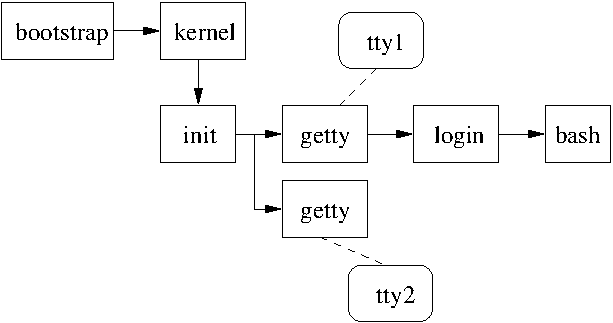
\includegraphics[width=\hsize]{init.pdf}\\

\end{frame}

\subsection{shell与进程}

\begin{frame}
\frametitle{Shell}

\begin{itemize}
\item shell的种类:
    \begin{itemize}
    \item Bourne shell : /bin/sh, 缺省提示符为 \$
    \item C shell: /bin/csh, 缺省提示符为 \%
	\item Korn shell : /bin/ksh, 缺省提示符为\$
    \item Bourne Again shell : /bin/bash, 缺省提示符为 \$
    \item Debian Almquist shell : 用于替换 /bin/sh的极简高效 shell
    \end{itemize}

\end{itemize}

\end{frame}


\begin{frame}
  \frametitle{Shell (cont.)}
\begin{itemize}
  \item shell命令形式
\begin{itemize}
\item Aliases
\item Functions (bash)
\item Built-in commands
\item Executable programs
\end{itemize}

\item shell命令搜索路径, 环境变量PATH

\end{itemize}

\end{frame}

\begin{frame}[containsverbatim]
\frametitle{Bash 启动}

\begin{enumerate}
\item login启动的是登录shell,
将首先搜索执行/etc/profile,然后按 \verb=~=/.bash\_profile,
\verb=~=/.bash\_login,
\verb=~=/.profile的顺序搜索执行找到的第一个文件

\item 交互shell将首先执行/etc/bash.bashrc, 然后执行\verb=~=/.bashrc文件
\end{enumerate}

\end{frame}

\begin{frame}[containsverbatim]
\frametitle{显示进程}

格式: \alert{ps} [选项] \\
显示当前所有进程的详细信息\\[1ex]
\begin{Verbatim}
caodg@debian:~$ ps -ef | less
\end{Verbatim}

查看谁登录了 \\
\begin{Verbatim}
caodg@debian:~$ w
caodg@debian:~$ who
\end{Verbatim}

我是谁?\\
\begin{Verbatim}
caodg@debian:~$ who am i
caodg@debian:~$ whoami
\end{Verbatim}


\end{frame}

\begin{frame}[containsverbatim]
\frametitle{调整进程优先级}

\alert{Unix进程优先级与优先数: 数越大, 优先级越低, 执行越慢}\\
格式: \alert{nice} -n [[command] arg]\\
调整待运行的程序的运行优先级, 只有超级用户能提高优先级\\[1ex]
例: 让某长时间执行的非重要程序以低优先级运行\\
\begin{Verbatim}
caodg@debian:~$ nice -10 non-critical-long-time-job
\end{Verbatim}


\end{frame}

\begin{frame}[containsverbatim]
\frametitle{调整进程优先级 (cont.)}
格式: \alert{renice} n pid \\
改变当前进程的优先级\\
例: 让进程exim4 (pid为12513)优先运行(只有root可以)\\
\begin{Verbatim}
debian:# renice -5 12513
\end{Verbatim}

例: 让用户long的所有进程低优先级运行\\
\begin{Verbatim}
debian:# renice +5 -u long
\end{Verbatim}


\end{frame}

\begin{frame}[containsverbatim]
\frametitle{进程发信号}

格式: \alert{kill} [--signalnumber] pid\\
缺省给进程发送TERM信号, 中止进程\\

\begin{tabular}{p{3cm}p{3cm}p{9cm}}\hline
Num & Name & Action\\ \hline
1 & HUP & 重起进程 \\
2 & INT & 中断 \\
3 & QUIT & 退出 \\
9 & KILL & 强制杀死(unblock)\\
15 & TERM & 软中止 \\ \hline
\end{tabular}\\


\end{frame}

\begin{frame}[containsverbatim]
\frametitle{向进程发信号}

例: 杀死进程trojan (pid为1254)\\
\begin{Verbatim}
debian:# kill -9 1254
\end{Verbatim}

例: 让apache2重新加载配置 \\
\begin{Verbatim}
debian:# kill -HUP 5538
\end{Verbatim}
\end{frame}

\section{文件}

\subsection{基本操作}

\begin{frame}
\frametitle{树形文件系统}

Unix的文件系统是树形层次结构\\
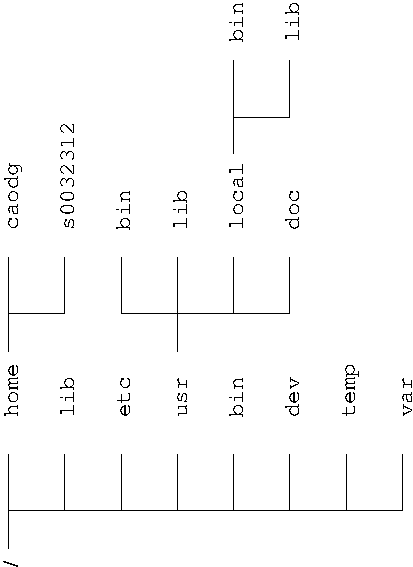
\includegraphics[scale=0.8,angle=-90]{directory.pdf}

\end{frame}

\begin{frame}
\frametitle{文件类型}
Unix系统有三种基本文件类型: 普通文件, 目录文件, 设备文件

\begin{itemize}

\item 套接字文件
\item 管道文件
\item 符号链接(指向另一个文件)
\item 块设备文件与字符设备文件
\item 目录文件
\item 普通文件: 文本文件与二进制文件
\end{itemize}

\end{frame}

\begin{frame}[containsverbatim]
\frametitle{目录}
\begin{itemize}
\item 系统根目录: \alert{/}
\item 当前目录,工作目录: \alert{.}
\item 当前目录的父目录: \alert{..}
\item 用户主目录(Home Directory): \verb=~=
  \end{itemize}
  
\end{frame}


\begin{frame}
  \frametitle{路径}
路径(Path): 从树形目录结构中的某个目录到某个文件的一条道路
\begin{itemize}
    \item 目录分隔符为``/'', 例如``/usr/bin/java''
    \item 绝对路径:从根开始的路径,也称为完全路径
    \item 相对路径:从用户工作目录开始的路径
\end{itemize}

\end{frame}

\begin{frame}[containsverbatim]
\frametitle{简单命令}

\begin{itemize}
\item 查看当前所在目录\\[0.5ex]
\begin{Verbatim}
caodg@debian:~$ pwd
/export/home/caodg
\end{Verbatim}

\item 查看当前目录内容\\[0.5ex]
\begin{Verbatim}
caodg@debian:~$ ls -F
a.c a.out* grade.txt bak/ java/ tex/
\end{Verbatim}

\end{itemize}


\end{frame}


\begin{frame}[containsverbatim]
\frametitle{简单命令 (cont.)}

\begin{itemize}
\item 进入子目录\\[0.5ex]
\begin{Verbatim}
caodg@debian:~$ cd java
caodg@debian:~/java$
\end{Verbatim}

\item 到上级目录\\[0.5ex]
\begin{Verbatim}
caodg@debian:~/java$ cd ..
\end{Verbatim}

\end{itemize}

\end{frame}


\begin{frame}
\frametitle{文件通配符}
\begin{itemize}
\item Unix的文件名可以为任意字符
\item 隐藏文件: 以``\alert{.}''开头的文件, 如 \alert{.bashrc}
\item 通配符\alert{\textbf{*}} : \alert{\textbf{*}}匹配非隐藏文件名中的任意字符串
\item 通配符\alert{\textbf{?}} : \alert{\textbf{?}}匹配非隐藏文件名中任意单个字符
\item 字符组\alert{\textbf{[字符组]}}, \alert{\textbf{[字符-字符]}}: 匹配中括号中的任一个,
\alert{\textbf{[!字符组]}}表示不匹配方括号中的任意字符
\item 转义字符\alert{\textbf{$\backslash$}} : \alert{\textbf{$\backslash$}}
让\alert{\textbf{*}},\alert{\textbf{?}},以及方括号中的\alert{\textbf{-}}失去通配符作用
\end{itemize}

\end{frame}

\begin{frame}[containsverbatim]
\frametitle{文件通配符示例}
\begin{itemize}
\item 列出当前目录下以abc开头的文件\\[1ex]
\begin{Verbatim}
caodg@debian:~$ ls abc*
abc  abcd  abc_d  abc.d
\end{Verbatim}

\item 列出当前目录下以abc结尾的文件\\[1ex]
\begin{Verbatim}
caodg@debian:~$ ls *abc
abc  aabc  a.abc  a.b.abc
\end{Verbatim}

\end{itemize}

\end{frame}

\begin{frame}[containsverbatim]
\frametitle{文件通配符示例 (cont.)}
\begin{itemize}

\item 列出以任意两个字符开头, 接着是R,
后面跟任何字符的文件\\[1ex]
\begin{Verbatim}
caodg@debian:~$ ls ??R*
abR  cdRc  RRR.abc
\end{Verbatim}

\item 列出文件名开头不是a或b或c或d的文件\\[1ex]
\begin{Verbatim}
caodg@debian:~$ ls [!a-d]*
e  fg  zz.sh
\end{Verbatim}

\end{itemize}

\end{frame}

\begin{frame}[containsverbatim]
\frametitle{文件复制}

格式: \alert{cp} [选项] SOURCES \quad DEST \\
\alert{cp}命令用于将一个文件复制为另一个文件,或将文件复制到另一目录

\begin{itemize}
\item 将文件aaa复制为bbb\\
\begin{Verbatim}
caodg@debian:~$ cp aaa bbb
\end{Verbatim}

\end{itemize}

\end{frame}

\begin{frame}[containsverbatim]
  \frametitle{文件复制}
  
  \begin{itemize}
\item 将所有C语言文件复制到bak目录\\
\begin{Verbatim}
caodg@debian:~$ cp *.c bak
\end{Verbatim}

\item 将aaa和bbb复制到bak目录\\
\begin{Verbatim}
caodg@debian:~$ cp aaa bbb bak
\end{Verbatim}

\item 将目录java递归复制到bak目录\\
\begin{Verbatim}
caodg@debian:~$ cp -r java bak
\end{Verbatim}

\end{itemize}

\end{frame}


\begin{frame}[containsverbatim]
\frametitle{文件删除}

格式: \alert{rm} [选项] FILES \\
\alert{rm}命令用于删除文件或目录,默认情况下\alert{rm}不删除目录

\begin{itemize}
\item 将所有.o文件删除, 删除前确认\\
\begin{Verbatim}
caodg@debian:~$ rm -i *.o
\end{Verbatim}

\end{itemize}

\end{frame}

\begin{frame}[containsverbatim]
  \frametitle{文件删除 (cont.)}

  \begin{itemize}
\item 将所有.o文件强制删除\\
\begin{Verbatim}
caodg@debian:~$ rm -f *.o
\end{Verbatim}

\item 将bak目录及其下所有文件强制删除\\
\begin{Verbatim}
caodg@debian:~$ rm -rf bak
\end{Verbatim}

\end{itemize}
小心: Unix中文件删除不可恢复!!


\end{frame}

\begin{frame}
    \frametitle{彻底删除文件}
    \begin{itemize}
        \item shred:  覆盖写以删除文件使之不可恢复
        \item srm:
        \item wipe:
    \end{itemize}
\end{frame}


\begin{frame}[containsverbatim]
\frametitle{文件移动}

格式: \alert{mv} [选项] SOURCE DEST \\
\alert{mv}命令用于将一个文件改名,或将文件移动到另一目录

\begin{itemize}
\item 将文件aaa更名为bbb\\
\begin{Verbatim}
caodg@debian:~$ mv aaa bbb
\end{Verbatim}

\item 将所有.o文件移动到tmp目录\\
\begin{Verbatim}
caodg@debian:~$ mv *.o tmp
\end{Verbatim}

\item 将文件aaa移动到bbb目录\\
\begin{Verbatim}
caodg@debian:~$ mv aaa bbb
\end{Verbatim}

\end{itemize}


\end{frame}

\begin{frame}[containsverbatim]
\frametitle{目录创建}

格式: \alert{mkdir} [-p] DIR \\
\alert{mkdir}命令用于创建一个目录

\begin{itemize}
\item 在当前目录创建目录bbb\\
\begin{Verbatim}
caodg@debian:~$ mkdir bbb
\end{Verbatim}

\item 在子目录bbb中创建目录ccc, 若bbb不存在, 一并创建\\
\begin{Verbatim}
caodg@debian:~$ mkdir -p bbb/ccc
\end{Verbatim}

\end{itemize}


\end{frame}

\begin{frame}[containsverbatim]
  \frametitle{目录删除}
  \begin{itemize}
	\item 用\alert{~rm~} 命令 , 带\alert{-r}参数 \\
\begin{Verbatim}
caodg@debian:~$ rm -r aaa
\end{Verbatim}

\item 用 \alert{rmdir} 命令删除空目录 \\
\begin{Verbatim}
caodg@debian:~$ rmdir aaa/bbb
\end{Verbatim}

\item \alert{rmdir -p} 删除空目录及父目录 \\
\begin{Verbatim}
caodg@debian:~$ rmdir -p aaa/bbb
\end{Verbatim}
等价于 \\
\begin{Verbatim}
caodg@debian:~$ rmdir aaa/bbb aaa
\end{Verbatim}
\end{itemize}


\end{frame}

\begin{frame}[containsverbatim]
\frametitle{目录查看}

格式: \alert{ls} [选项] FILES \\
\alert{ls}命令用于查看文件或目录的信息

\begin{itemize}
\item 列出当前目录所有文件的详细信息, 包括隐藏文件\\
\begin{Verbatim}
caodg@debian:~$ ls -al
\end{Verbatim}

\item 列出当前目录所有文件的详细信息, 按照修改时间排序\\
\begin{Verbatim}
caodg@debian:~$ ls -tl
\end{Verbatim}

\end{itemize}


\end{frame}


\begin{frame}[containsverbatim]
\frametitle{目录查看 (cont.)}

\begin{itemize}

\item 列出当前目录及其子目录所有文件的详细信息\\
\begin{Verbatim}
caodg@debian:~$ ls -Rl
\end{Verbatim}

\item 显示文件类型: \\
  *可执行, /目录, @符号连接, $|$管道, =套接字\\
\begin{Verbatim}
caodg@debian:~$ ls -F
\end{Verbatim}

\end{itemize}

\end{frame}

\subsection{进阶操作}

\begin{frame}[containsverbatim]
\frametitle{文件权限}

{\Large{\verb=rwxr-xr--=}}

9个字符表示权限位,其中
\begin{description}
\item [rwx]: 前三位表示文件属主有读写执行权限
\item [r-x]: 中间三位表示用户所在组有读和执行权限
\item [r-{}-]: 后三位表示其它用户有读权限
\end{description}

可以用二进制表示: 111\alert{101}100

\end{frame}

\begin{frame}[containsverbatim]
\frametitle{修改文件权限}

格式: \alert{chmod} [选项] MODE[,MODE], FILES \\
MODE可为8进制,或者[augo] [+--=] [rwx]

\begin{itemize}
\item 让所有用户都可执行a.sh文件\\
\begin{Verbatim}
caodg@debian:~$ chmod a+x a.sh
\end{Verbatim}

\item 让属主具有执行权限\\
\begin{Verbatim}
caodg@debian:~$ chmod u+x a.sh
\end{Verbatim}

\end{itemize}


\end{frame}

\begin{frame}[containsverbatim]
\frametitle{修改文件权限 (cont.)}

\begin{itemize}
\item 去掉组用户的写权限, 增加其他用户的读权限\\
\begin{Verbatim}
caodg@debian:~$ chmod g-w,o+r a.sh
\end{Verbatim}

\item 设定所有文件的权限为属主读写执行,组读执行,其他读\\
\begin{Verbatim}
caodg@debian:~$ chmod -R 754 a.sh
\end{Verbatim}

\end{itemize}
\end{frame}

\begin{frame}[containsverbatim]
    \frametitle{控制新创建文件的缺省权限: umask}
\begin{verbatim}    
     文件权限 = (请求创建的文件权限) & ~(umask value)
 \end{verbatim}

 \begin{tabular}{ c | c | c | l}
     \hline
     umask & 新文件的权限 & 新目录的权限 & 用处 \\
     \hline \hline
     0022 &  -rw-r--r--  & -rwxr-xr-x  & 属主可写 \\
     0002 &  -rw-rw-r--  & -rwxrwxr-x  & 组可写  \\
     \hline
 \end{tabular}
\end{frame}

\begin{frame}[containsverbatim]
\frametitle{suid和guid}

问题:
/etc/passwd文件对普通用户不可写,但是用户执行passwd命令后,可以更新/etc/passwd文件中自己的密码,如何实现?\\
答案: suid/guid

\begin{Verbatim}
-rwsr-xr-x  1 root root 26616 May 18 2005 /usr/sbin/passwd
\end{Verbatim}

设置suid/guid示例: 为a.sh文件设置suid/guid位\\
\begin{Verbatim}
caodg@debian:~$ chmod u+s,g+s a.sh
\end{Verbatim}
有比较严重的安全隐患
\end{frame}

\begin{frame}
\frametitle{有效用户与实际用户}

\begin{itemize}
\item 实际(real)用户id: 进程的属主,谁在运行该程序, 用于记帐
\item 实际组id: 
\item 有效(effective)用户id: 进程在运行时的权限
\item 有效组id: 
\end{itemize}
\end{frame}



\begin{frame}[containsverbatim]
\frametitle{改变文件时间}

格式: \alert{touch} [选项] FILES \\
\alert{touch}命令用于修改文件的访问时间和修改时间,默认情况下为当前时间,如果文件不存在,则创建该文件

\begin{itemize}
\item 将文件a.sh的时间修改为当前时间\\
\begin{Verbatim}
caodg@debian:~$ touch a.sh
\end{Verbatim}

\item 将文件a.sh的时间修改为2006年3月8日16时50分\\
\begin{Verbatim}
caodg@debian:~$ touch -t 200603081650
\end{Verbatim}

\item 创建一个新文件b.sh\\
\begin{Verbatim}
caodg@debian:~$ touch b.sh
\end{Verbatim}

\end{itemize}



\end{frame}

\begin{frame}
\frametitle{文件链接}

\begin{itemize}
\item 硬链接(hard link): 一个文件是另一个文件的别名, 是一个文件实体
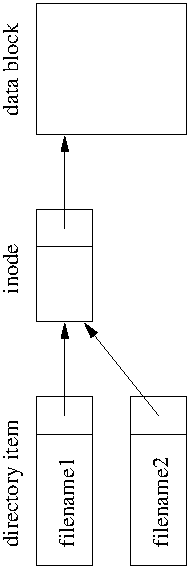
\includegraphics[scale=1.0,angle=-90]{ln.pdf}
\begin{itemize}
\item 不能指向目录
\item 不能跨越文件系统
\end{itemize}

\end{itemize}


\end{frame}

\begin{frame}
\frametitle{文件链接}

\begin{itemize}
\item 软链接(symbolic link):符号链接, 内容指向链接目标文件名
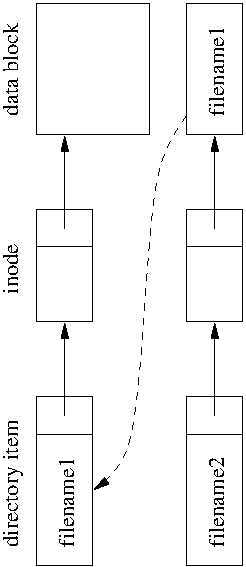
\includegraphics[scale=1.0,angle=-90]{lns.pdf}
\begin{itemize}
\item 可以链接目录
\item 可以跨越文件系统
\end{itemize}
\end{itemize}


\end{frame}

\begin{frame}[containsverbatim]
\frametitle{文件链接操作}

格式: \alert{ln} [选项] SOURCE DEST \\
\alert{ln}命令用于创建一个从SOURCE到DEST的链接

\begin{itemize}
\item 为文件a.cc产生一个符号链接a.ln\\[1ex]
\end{itemize}
\begin{Verbatim}
caodg@debian:~$ ln -s a.cc a.ln
caodg@debian:~$ ls -il
 342058 -rw-r--r-- 1 caodg caodg 0 Mar 6 2006 a.cc 
 342059 lrwxrwxrwx 1 caodg caodg 4 Mar 6 2006 a.ln --> a.cc
\end{Verbatim}
 
\end{frame}

 \begin{frame}[containsverbatim]
   \frametitle{文件链接操作}

\begin{itemize}
\item 为文件a.cc产生一个硬链接a.ln\\[1ex]
\end{itemize}

\begin{Verbatim}
caodg@debian:~$ ln a.cc a.ln
caodg@debian:~$ ls -il
 342058 -rw-r--r-- 1 caodg caodg 0 Mar 6 2006 a.cc
 342058 -rw-r--r-- 1 caodg caodg 0 Mar 6 2006 a.ln
\end{Verbatim}

\end{frame}

\begin{frame}[containsverbatim]
\frametitle{查看文本文件内容}
格式: \alert{cat} [选项] FILES

例: 显示a.cc的内容, 给每行加上行号\\[1ex]
\begin{Verbatim}
caodg@debian:~$ cat -n a.cc
 1 int myChl (char *p)
 2 {
 3	char r;
 4	int i;
 5	return 0;
 6 }
\end{Verbatim}
\end{frame}


\begin{frame}[containsverbatim]
\frametitle{分页显示文本文件内容}

格式: \alert{more} [选项] FILES \\
格式: \alert{less} [选项] FILES \\

命令\alert{less}是\alert{more}的增强版, 提供更多的控制选项和更好的性能.

\alert{less}和\alert{more}经常和其它命令通过管道机制结合使用.\\[1ex]
例: 分页显示/usr/bin目录下的文件信息\\
\begin{Verbatim}
caodg@debian:~$ ls -l /usr/bin | more
\end{Verbatim}
\end{frame}

\begin{frame}
\frametitle{less}

less的基本控制命令:
\begin{itemize}
\item 空格: 向前翻页, 同Ctrl + f
\item 回车: 向前一行
\item Ctrl+b: 向后翻页
\end{itemize}


\end{frame}

\begin{frame}[containsverbatim]
\frametitle{统计单词}

格式: \alert{wc} [选项] FILES \\
\alert{wc}命令缺省情况下输出文件的行数, 单词数, 字符数

\begin{itemize}
\item 统计a.cc的行数, 单词数, 字符数\\[1ex]
\begin{Verbatim}
caodg@debian:~$ wc a.cc
7 14 159 a.cc
\end{Verbatim}

\item 统计a.cc的行数\\[1ex]
\begin{Verbatim}
caodg@debian:~$ wc -l a.cc
7 a.cc
\end{Verbatim}

\end{itemize}

\end{frame}

\begin{frame}[containsverbatim]
  \frametitle{归档}
命令: \alert{tar}

\begin{itemize}
\item 将java目录归档为java.tar文件\\
\begin{Verbatim}
caodg@debian:~$ tar cvf java.tar java
\end{Verbatim}

\item 释放java.tar文件\\
\begin{Verbatim}
caodg@debian:~$ tar xvf java.tar
\end{Verbatim}

\item 显示java.tar文件中的内容\\
\begin{Verbatim}
caodg@debian:~$ tar tvf java.tar
\end{Verbatim}

\end{itemize}

\end{frame}


\begin{frame}
\frametitle{压缩与解压缩}
各种命令: 
\begin{itemize}
  \item \alert{gzip}, \alert{gunzip} : .gz, .z
  \item \alert{zip}, \alert{unzip} : .zip 
  \item \alert{bzip2}, \alert{bunzip2}: .bz2
  \item \alert{unrar}, \alert{p7zip}: .rar, .7z
\end{itemize}


\end{frame}

\begin{frame}[containsverbatim]
\frametitle{压缩与解压缩示例}

\begin{itemize}

\item 将java目录归档并压缩\\
\begin{Verbatim}
caodg@debian:~$ tar cvfz java.tgz java
\end{Verbatim}

\item 释放java.tgz文件\\
\begin{Verbatim}
caodg@debian:~$ tar xvfz java.tgz
\end{Verbatim}

\end{itemize}
\end{frame}

\section{其他}

\subsection{网络操作}

\begin{frame}
\frametitle{ftp}

基本的ftp访问操作
\begin{itemize}
\item 输入用户名密码: user
\item 设置传输方式: asc, bin
\item 单个传输: get, put
\item 批量传输: mget, mput, prompt
\end{itemize}
\end{frame}

\begin{frame}
\frametitle{lftp}
lftp: 提供类似sh的语法, 支持tab补齐, 下载目录(mirror)等, 非常强大
\begin{itemize}
  \item 递归下载一个目录: mirror
  \item 递归上传一个目录: mirror -R
  \item 站点管理: bookmark
  \item 任务排队: queue
\end{itemize}
\end{frame}

\begin{frame}[containsverbatim]
\frametitle{WWW浏览}

命令: lynx 和 w3m

\begin{itemize}
\item 面向字符终端的纯文本界面
\item 功能完全的WWW客户端
\item 可以下载文件
\item 可以浏览组织本地文件
\end{itemize}

\begin{Verbatim}
caodg@debian:~$ w3m www.pku.edu.cn
\end{Verbatim}

\begin{Verbatim}
caodg@debian:~$ w3m /
\end{Verbatim}


\end{frame}

\begin{frame}
\frametitle{聊天}

\begin{itemize}
\item 命令\alert{talk}支持跨机器的两个用户的谈话

例如: Machine A上的用户user1要talk Machine B上的用户user2\\
user1: talk user2@B\\
user2: talk user1@B

\item 命令\alert{write}用于同一主机上的用户之间发送消息

\item 命令\alert{wall}用于向所有用户广播消息

\item 命令\alert{mesg}用于打开接受消息开关
\end{itemize}


\end{frame}

\begin{frame}
  \frametitle{Internet聊天}
  IRC (Internet Relay Chat)
  \begin{itemize}
	\item 1988年起源于芬兰
	\item 是talk的替代工具, 但功能远远超出
	\item 可设频道, 共享信息, 可私密谈话
	\item 支持文件传输
	\item 广泛应用于开源开发者中
	\item 主要分为欧洲和北美两大风格
  \end{itemize}
  
\end{frame}

\begin{frame}
\frametitle{文件下载: wget, axel}

命令: wget [OPTIONS] [URL]

\begin{itemize}
\item 支持HTTP, HTTPS, FTP协议
\item 支持断点续传
\item 可以镜像整个/部分web站点
\end{itemize}


\end{frame}

\begin{frame}[containsverbatim]
\frametitle{文件下载}

下载一个文件\\
\begin{Verbatim}
caodg@debian:~$ wget http://x.y.cn/chap01.pdf
\end{Verbatim}

递归下载一个ftp目录\\
\begin{Verbatim}
caodg@debian:~$ wget -rc ftp://x.y.cn/bc
\end{Verbatim}

断点重传上次没下载完的目录\\
\begin{Verbatim}
caodg@debian:~$ wget -rc ftp://x.y.cn/bc
\end{Verbatim}

下载课程网页及其所有本地文件\\[1ex]
\begin{Verbatim}
caodg@debian:~$ wget -r -k -np 
  http://www.sei.pku.edu.cn/~caodg/course/unix
\end{Verbatim}

 
\end{frame}

\subsection{其他}

\begin{frame}[containsverbatim]
\frametitle{时间}
格式: \alert{date} [选项]\\
缺省显示当前时间

\begin{itemize}
\item 查看当前时间\\[1ex]
\begin{Verbatim}
caodg@debian:~$ date
\end{Verbatim}

\item 设置当前时间为2006年3月7日15时20分\\[1ex]
\begin{Verbatim}
caodg@debian:~$ date 030715202006
\end{Verbatim}

\end{itemize}


\end{frame}

\begin{frame}[containsverbatim]
  \frametitle{日历}

命令\alert{cal}显示日历
\begin{itemize}
\item 显示2006年日历\\[1ex]
\begin{Verbatim}
caodg@debian:~$ cal 2006
\end{Verbatim}
\end{itemize}

命令\alert{lunar}进行农历和公历转换
\begin{itemize}
\item  查询公元2007年10月1日的农历日期 \\
\begin{Verbatim}
caodg@debian:~$ lunar -h 2007 10 1
\end{Verbatim}
\item  查询农历2008年1月1日的公历 \\
\begin{Verbatim}
caodg@debian:~$ lunar -h -i 2008 1 1
\end{Verbatim}

\end{itemize}

 
\end{frame}

\begin{frame}[containsverbatim]
\frametitle{词典和拼写检查}
查词典: \alert{dict}, \alert{cdict}, \alert{wn}\\
拼写检查: \alert{aspell}, \alert{spell}

\begin{itemize}
\item 查看``philosophy''的解释\\[1ex]
\begin{Verbatim}
caodg@debian:~$ dict philosophy
\end{Verbatim}

\item 查看``philosophy''的中文解释\\[1ex]
\begin{Verbatim}
caodg@debian:~$ cdict philosophy
\end{Verbatim}

\item 拼写检查myletter.txt\\[1ex]
\begin{Verbatim}
caodg@debian:~$ aspell -c letter.txt
caodg@debian:~$ spell letter.txt
\end{Verbatim}

\end{itemize}


\end{frame}



\begin{frame}
\frametitle{计算器}
格式: \alert{bc} [选项] [文件]\\

\begin{itemize}
\item 任意精度
\item 数学库,支持$\arctan{x}$, $\sin{x}$, $\ln{x}$等
\item 各种数学,逻辑运算符
\item 控制语句,循环, 赋值
\item 自定义变量,函数
\end{itemize}


\end{frame}

\begin{frame}[containsverbatim]
\frametitle{$2^{5555}=$}

\begin{tabular}{|l|}\hline
\begin{minipage}{0.9\hsize}
\vspace{2mm}\tiny
\renewcommand{\baselinestretch}{1.1}
\begin{verbatim}
16658117204979357086011751763732109295737684996665146016607920416687\
54246194216415068056761548789905430869964396196359597235190154495115\
83490301210210840360839330879454490129431062428594199611824466845894\
92432481329632844309689388555386482122756325762769501532493681143469\
59621021518840634099457216046357178455556428503206618269979586068248\
72234434011792001180542678060468086893393162905399110596090102876141\
29787680369584033288759793734410797618006233391180065497826928163406\
58218763549538837576485798342839741629904255636530495888723173508639\
76006716212214314668645258858606031470084984782627481917057316292741\
59115294019456772453885127094553464734246597872439543614614100569719\
40055206105856212416991485135881787249255651026567089928201844330191\
34571071847200268914511912520597125117548568566946483030997136420491\
41136905869439487048096656287611550827771125381190492470234808930560\
07234836131667423171834493242148297004314173805051211197302586860882\
09610699459288073814900859395919077197628894321452096486994293320388\
81637110504699757309590231678079955629244528883714234409096407607065\
49795942294045577686960199138240276891569610225401336417392536570548\
12355686060354578881555784933622821558219249496707892321413995725491\
47688684029652822764209520195405572055996412444549778644759583591630\
85365958922442895705482569889998140077739073146087660079594446510685\
47314076978843943379756801126392959235574191774932737100213986451256\
60682407922801393001478854129924492363784484065306420565410942156987\
12220782800682124468294824352927442653012919494414720485035718979953\
85263613380383518425806065486567965431503024493272508540999392203492\
66024875689347184740241634715530290003968
\end{verbatim}
\vspace{1mm}
\end{minipage}\\
\hline
\end{tabular}
\end{frame}


\begin{frame}
\frametitle{帮助}
格式: \alert{man} [选项] [[节] page] \\
page可以是程序名, 系统调用名, 库函数名, 等等. page按节归类:

\begin{enumerate}
\item   Executable programs or shell commands
\item   System calls (functions provided by the kernel)
\item   Library calls (functions within program libraries)
\item   Special files (usually found in /dev)
  \end{enumerate}
  
\end{frame}


\begin{frame}
\frametitle{帮助}
\begin{enumerate}
\setcounter{enumi}{4}
\item   File formats and conventions eg /etc/passwd
\item   Games
\item   Miscellaneous  (including  macro  packages and conventions), e.g. man(7), groff(7)
\item   System administration commands (usually only for root)
\item   Kernel routines [Non standard]
\end{enumerate}

例如,查看man的用法: \alert{man man}
 
\end{frame}

\begin{frame}
\frametitle{其它有用命令}
\begin{itemize}
\item \alert{du}: 查看文件/目录占用磁盘空间
\item \alert{df}: 查看磁盘分区
\item \alert{uname}: 查看操作系统信息
\item \alert{which}: 查看命令的全路径
\item \alert{top}: 实时查看进程信息
\item \alert{nano}: Debian自带的一个简单编辑器
\item \alert{info}: GNU的帮助系统

\end{itemize}

\end{frame}

\end{document}
